\chapter{基于内存压力的自动卸载框架}
\label{chap:基于内存压力的自动卸载框架}

在\ref{chap:基于同步内存回收的内存压力量化算法的设计与实现}中,本研究将同步内存回收延迟量化为内存压力指标。基于该量化指标,用户态的内存压力感知卸载框架能够主动将冷页面卸载到异构后端存储设备。本章将详细介绍基于proc文件系统的mpfs(内存压力文件系统)实现、基于内存压力的工作集动态估计算法,以及基于重用的匿名页和文件页自适应平衡回收策略的设计与实现。




\section{内存压力文件系统的实现}
\label{sec:mpfs_implementation}

基于\ref{sec:基于同步回收延迟的内存压力量化实现}节实现的内存压力量化模型,本节构建用户态调控接口,实现系统内存资源的动态管理机制。内存压力量化提供了关键的系统状态指标,建立在此基础上的负反馈调节系统需要灵活的策略支持,以响应动态变化的资源状况。

选择在用户态实现内存压力响应策略主要基于以下理论依据与技术考量:

\begin{itemize}
    \item 策略复杂性与迭代速度:用户态环境支持实现复杂的调控策略,同时具备较短的开发、测试和部署周期,便于快速迭代优化。
    \item 差异化服务质量保障:不同应用程序对内存资源的敏感度和优先级存在差异,用户态实现便于针对特定QoS需求定制差异化的资源分配策略。
    \item 运行时可配置性:支持在系统运行过程中动态调整策略参数,无需重新编译或加载内核模块。
\end{itemize}

本节设计的内存压力文件系统(Memory Pressure File System, mpfs)构建了内核与用户态策略引擎之间的标准化通信接口,形成了完整的信息反馈与控制通道。

\subsection{proc文件系统架构分析}

proc文件系统作为Linux系统中内核与用户空间交互的标准机制,具备若干使其成为实现跨内核态与用户态内存压力信息交互理想媒介的特性。其动态生成机制使文件节点能够根据内核运行时状态实时动态构建;虚拟存储特性意味着不占用物理存储空间,通过内存映射实现数据存取;双向交互能力支持通过标准I/O系统调用进行内核参数查询与配置;抽象访问层则对用户态程序隐藏内核数据结构的复杂性,提供统一的访问接口。这些特性使得proc文件系统特别适合作为内核态与用户态进行内存状态交互的媒介。

\subsection{mpfs系统架构设计}

本研究设计的 mpfs 实现了三个核心功能接口: /proc/mpfs/mem\_pressure 提供实时内存压力值轮询接口并支持事件驱动的通知机制; /proc/mpfs/period 提供采样周期动态可配置接口(时间单位:秒); /proc/mpfs/mthreshold 提供修改触发阈值接口(百分比形式)。表\ref{tab:mpfs_files}详细描述了各文件接口的操作语义及功能映射关系。

\begin{table}[htbp]
    \centering
    \caption{mpfs文件系统接口规范}
    \label{tab:mpfs_files}
    \begin{tabular}{lccc}
        \toprule
        \textbf{操作类型} &  mem\_pressure  &  period  &  mthreshold  \\
        \midrule
         read  & 读取当前压力值 & 获取采样周期 & 查询当前阈值 \\
         write  & - & 更新采样周期 & 修改触发阈值 \\
         poll  & 事件通知机制 & - & - \\
        \bottomrule
    \end{tabular}
\end{table}

\begin{figure}[htbp]
  \centering
  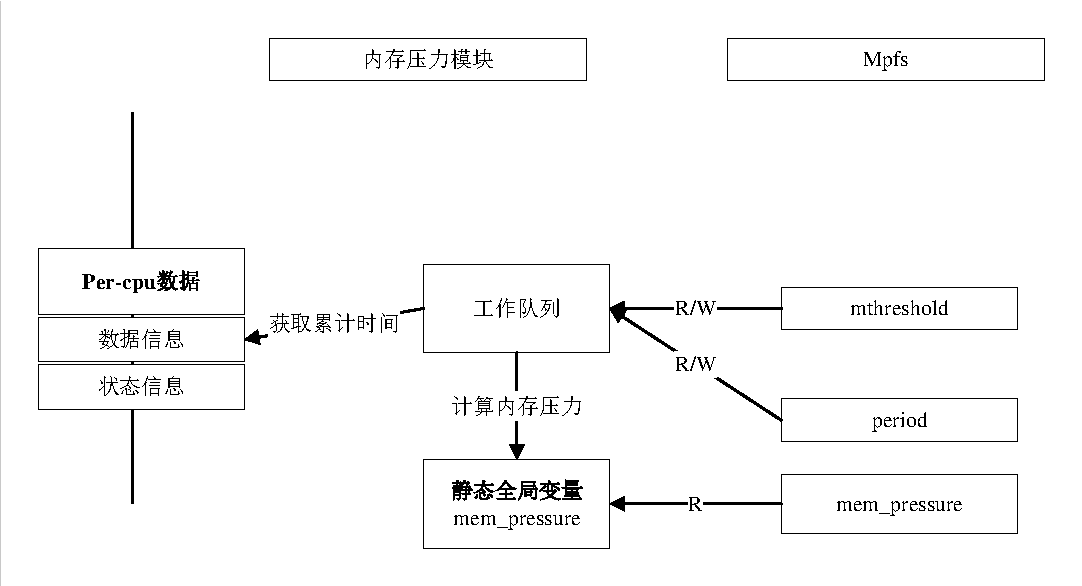
\includegraphics[width=\textwidth]{mpfs.pdf}
  \caption{mpfs与内存压力模块的交互}
  \label{fig:mpfs}
\end{figure}

图\ref{fig:mpfs}显示了mpfs和内存压力模块的交互。 mem\_pressure 接口在读取操作时访问内存压力模块中的静态全局变量以获取最新的内存压力值。对于采样周期的读写都是对内存压力模块中的工作队列进行配置,在第\ref{sec:consumer_implementation}节中,系统采用工作队列作为消费者,周期性执行压力计算任务。所以实际是在配置这个。 mthreshold  的读写也是在配置工作队列中的变量,因为每次在计算完成压力之后我们需要唤醒等待的进程。

\subsection{内核模块实现细节}

mpfs内核模块实现基于Linux内核的proc文件系统接口机制,遵循内核模块的加载与卸载生命周期,同时提供线程安全的内存压力数据访问。以下详细阐述其核心组件设计与实现策略。

\subsubsection{文件节点与操作接口}

mpfs为用户态程序提供三个主要的proc文件接口,每个接口对应特定功能,如表\ref{tab:mpfs_files_description}所示。这些接口通过标准的 file\_operations 结构与相应的处理函数绑定,提供一致的访问语义。

\begin{table}[htbp] % 使用 table 环境,使其成为浮动体
  \centering % 将 \centering 放在 table 环境内部
  \caption{mpfs 文件节点功能说明}
  \label{tab:mpfs_files_description}
  \begin{tabularx}{\textwidth}{cX} % 使用 tabularx,并用 X 列类型
      \toprule
      \textbf{文件节点} & \textbf{功能说明} \\
      \midrule
       /proc/mpfs/mem\_pressure  & 提供内存压力值读取和事件通知功能。
      读取操作返回当前压力百分比,poll 操作支持阻塞等待压力阈值突破事件。 \\
       /proc/mpfs/period  & 提供采样周期配置接口。读取操作返回当前采样周期(秒),写入操作允许动态调整采样周期。 \\
       /proc/mpfs/mthreshold  & 提供阈值配置接口。读取操作返回当前触发阈值(百分比),写入操作允许动态设置触发阈值。 \\
      \bottomrule
  \end{tabularx}
\end{table}

读取函数通过 sprintf 格式化当前值,并使用 copy\_to\_user 安全地传递到用户空间。函数设计考虑了文件偏移量( ppos )管理,确保多次读取的正确行为。写入函数执行严格的输入验证,确保数值在有效范围内(如阈值在0-100之间),通过 kstrtofl 函数进行安全的字符串到浮点数转换,避免溢出和格式错误。

轮询函数 mempressure\_poll 通过Linux内核的等待队列机制实现事件驱动的通知模型。当用户态进程通过poll系统调用监测内存压力文件时,该函数将调用进程添加到等待队列中;当工作队列周期性计算检测到压力值超过阈值时,工作函数设置标志位并唤醒队列上的所有进程,使它们能够读取最新的压力值并执行相应策略。此设计有效避免了用户态进程频繁轮询的资源开销,提升了系统的监测效率。

\subsubsection{模块初始化与资源管理}

模块初始化函数( mpfs\_init )负责构建完整的文件系统结构。执行过程首先创建 /proc/mpfs 目录作为挂载点,然后在该目录下创建三个文件节点,并绑定相应的文件操作函数集。随后初始化单线程工作队列,避免多线程竞争带来的复杂性,并设置默认配置参数(采样周期和触发阈值)。最后调度第一次工作,启动监测循环。相应地,模块卸载函数( mpfs\_exit )负责完整的资源释放,先取消并等待所有挂起的工作完成,然后销毁工作队列,最后移除所有创建的proc文件条目。这种严格的资源管理策略确保了模块在加载和卸载过程中的稳定性和可靠性。

\subsubsection{错误处理与安全机制}

mpfs实现了全面的错误处理机制,确保系统在各种异常情况下的稳定运行。在模块初始化过程中,遵循分层式资源释放原则,任何步骤失败都会按照创建顺序的逆序释放已分配资源,有效避免资源泄漏现象。例如,在工作队列创建失败时,会自动清理已创建的proc文件节点,保持系统状态一致性。

针对用户输入安全,模块对所有通过proc文件接口传入的配置参数进行严格验证。采样周期被限制在1-600秒的范围内,阈值被约束在0-100的百分比区间,通过 kstrtofl 函数安全地将字符串转换为浮点数,防止格式错误和溢出。对于恶意输入,模块返回明确的错误码,确保即使在异常输入条件下也能维持正常运行。

为应对多核环境下的竞态挑战,关键状态更新全部采用原子操作机制。内存压力百分比和触发标志通过 atomic\_set 和 atomic\_read 函数进行操作,避免了多处理器环境下数据不一致的风险。此外,用户空间与内核空间的数据交换严格通过 copy\_to\_user 和 copy\_from\_user 函数进行,防止直接指针访问可能导致的内核内存泄露或非法访问,提供了有效的安全防护机制。

这些安全机制深度集成于各个操作函数中,形成一个多层次的防护网络,从用户输入的边界检查,到内核内部的状态保护,再到资源管理的完整性保障,mpfs通过系统化的安全设计确保在高负载、频繁访问甚至恶意使用的复杂环境下保持健壮性和稳定性。

\subsection{用户态接口应用模式}

mpfs设计的核心价值在于为用户态策略引擎提供高效且易用的系统状态访问机制。典型的使用模式包含三个主要阶段:配置阶段,应用程序通过写入配置文件设置期望的监测参数,如采样周期和触发阈值;监测阶段,应用程序通过 poll 系统调用阻塞等待压力事件,或通过周期性读取获取实时压力值;响应阶段,当接收到压力事件通知后,应用程序执行相应的资源管理策略,如内存页面卸载或应用优先级调整。

以下伪代码展示了一个简洁的用户态监测应用示例:

\begin{lstlisting}[language=C]
// 配置阶段
int fd = open("/proc/mpfs/mem_pressure", O_RDONLY);
int thfd = open("/proc/mpfs/mthreshold", O_WRONLY);
write(thfd, "5.0", 3);  // 设置5.0%为触发阈值
close(thfd);

// 监测与响应阶段
struct pollfd pfd = {fd, POLLIN, 0};
while (running) {
    // 阻塞等待内存压力事件
    poll(&pfd, 1, -1);
    if (pfd.revents & POLLIN) {
        // 读取内存压力值并执行响应策略
        float pressure;
        read(fd, &pressure, sizeof(float));
        execute_memory_management_policy(pressure);
    }
}
close(fd);
\end{lstlisting}

这种设计模式将系统状态监测与策略执行分离,使得用户态程序能够根据特定场景需求实现定制化的资源管理策略,同时不需要关心低层次的数据采集细节。通过事件驱动的监测机制,系统资源开销得到有效控制,适合在各种负载条件下长期稳定运行。

\section{基于内存压力的动态调控模型}
\label{sec:pressure_based_model}

传统的工作集估计算法主要依赖于内存分配计数器、回收事件计数器等间接指标,这些方法的有效性受限于对存储硬件特性与内核行为的专业认知要求。为解决这一问题,第\ref{chap:基于同步内存回收的内存压力量化算法的设计与实现}章节提出了基于同步内存回收延迟的内存压力指标,该指标在不同负载模式和异构存储架构条件下表现出良好的通用性,克服了传统方法在特定场景适用性不足的缺陷。本节在此基础上,构建了一种基于内存压力的动态调控模型。该模型通过持续监测系统内存压力指标,实施主动回收策略,将低访问频率的数据页迁移至基于frontswap的异构存储后端,在满足性能约束条件下,优化内存资源利用效率。

\begin{figure}[h]
\centering
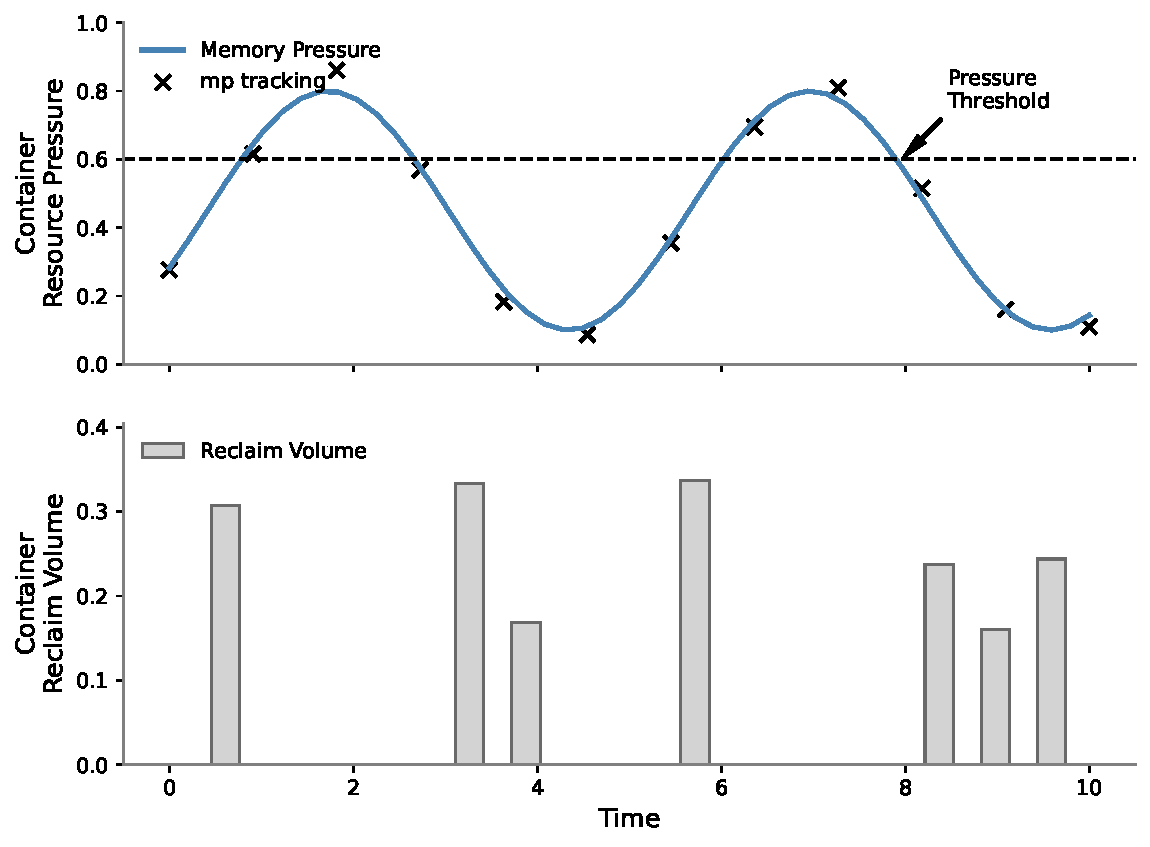
\includegraphics[width=0.95\textwidth]{压力与回收.pdf}
\caption{内存压力与页面回收调控机制}
\label{fig:pressure_work_set}
\end{figure}

图\ref{fig:pressure_work_set}展示了本模型的核心设计目标及运行机制。通过建立一个压力感知的闭环调控系统,该模型能够根据测量的内存压力值动态调整内存使用边界。当系统内存压力超过预设阈值时,模型逐步放宽内存限制以应对增长的工作集需求;反之,当内存压力低于目标值时,模型主动收紧内存限制并触发冷页面卸载,从而释放未充分利用的内存资源。这种基于压力的负反馈机制确保了系统能够在不同负载条件下维持接近最优的内存分配状态。

从经典反馈控制理论的视角看,本模型实现了闭环控制系统,以内存压力作为系统状态反馈,以内存分配大小为控制量,通过算法\ref{alg:control}动态调整控制输出。

\begin{table}[H]
\centering
\caption{调控参数体系}
\label{tab:params}
\begin{tabular}{cccc}
\toprule
参数名称 & 符号 & 默认值 & 作用域 \\
\midrule
目标压力 & \(mem\_pressure\_target\) & 0.1\% & 全局基准值 \\
最大收缩率 & \(M_p\) & 0.01 & 缩容阶段限制 \\
最大扩张率 & \(M_b\) & 1.0 & 扩容阶段限制 \\
收缩灵敏度 & \(C_p\) & 10 & 缩容函数参数 \\
扩张灵敏度 & \(C_b\) & 20 & 扩容函数参数 \\
\bottomrule
\end{tabular}
\end{table}

表\ref{tab:params}列出了算法的关键参数体系,这些参数直接对应算法\ref{alg:control}中的控制变量。目标压力值(\(mem\_pressure\_target\))作为全局调控基准,默认设置为0.1\%,表示系统期望维持的内存压力。灵敏度系数(\(C_p\)和\(C_b\))控制系统对压力变化的响应程度:扩张灵敏度\(C_b = 20\)表示当实际压力达到目标值20倍时,触发最大扩容比例;收缩灵敏度\(C_p = 10\)表示当压力降至目标值1/10时,系统执行最大缩容操作。最大调整率参数(\(M_b\)和\(M_p\))限定了单次调整的幅度上限:最大扩张比例\(M_b = 1.0\)允许在单次调整中将内存限制扩大至原值的两倍,以快速响应突发性工作负载;最大收缩比例\(M_p = 0.01\)将单次缩容限制在1\%以内,确保系统稳定性并避免服务质量剧烈波动。

算法\ref{alg:control}详细描述了基于压力量化的动态调控机制。与传统的静态内存分配策略不同,该算法通过实时内存压力指标构建了资源分配的动态反馈系统。算法以固定的时间间隔(默认为6秒)执行一次评估,通过计算当前内存压力与目标压力阈值之间的偏差来确定调整策略和幅度。

核心调整函数采用二次函数非线性映射(第6行和第10行)将压力偏差转换为调整系数,这一设计有几个关键优势:首先,二次函数在原点附近的梯度较小,使系统对接近目标值的小偏差不过度反应,避免了因测量噪声导致的抖动;其次,当偏差增大时,二次函数的响应强度快速提升,确保对显著偏离目标状态的情况能够做出迅速响应;最后,通过\(min\)函数对调整系数进行上界约束,防止过度调整导致的系统不稳定。与简单的线性映射相比,这种非线性映射在小偏差时抑制了系统过度反应,显著偏差时又能迅速响应,从而在不同工况下表现出更好的适应性与抗干扰能力。

\begin{algorithm}[htbp]
  \caption{Memory Pressure-Based Dynamic Control Algorithm}
  \label{alg:control}
  \Input{\(mem\_pressure\), \(mem\_pressure\_target\), \(C_b\), \(C_p\), \(M_b\), \(M_p\), \(min\_size\), \(max\_size\)}
  \Output{Memory Limit \(Limit\)}
  \While{true}{
      \(mem\_pressure \leftarrow\) Read current pressure value from procfs interface\;
      \If{\(mem\_pressure > mem\_pressure\_target\)}{
          \(\eta \leftarrow \min\left(\left(\frac{mem\_pressure/mem\_pressure\_target}{C_b}\right)^2, 1\right) \cdot M_b\)\;
          \(Limit \leftarrow \min(max\_size, Limit \times (1 + \eta))\)\;
      }
      \Else{
          \(\eta \leftarrow \min\left(\left(\frac{mem\_pressure\_target/mem\_pressure}{C_p}\right)^2, 1\right) \cdot M_p\)\;
          \(Limit \leftarrow \max(min\_size, Limit \times (1 - \eta))\)\;
      }
      Apply new memory limit \(Limit\)\;
      Wait for next sampling period (default: 6 seconds)\;
  }
\end{algorithm}


需要强调的是,上述算法设计具有高度可配置性,允许根据不同应用场景和性能需求进行参数调整。在高实时性要求的环境中,可以配置较高的扩张灵敏度和较低的收缩灵敏度,实现对压力增长的快速响应;而在资源受限且对性能波动容忍度较高的场景中,则可采用更积极的收缩策略以最大化资源利用率。通过这种参数化设计,算法能够适应从延迟敏感型在线服务到吞吐量导向的批处理任务等各类应用的负载特性。

此调控模型的优势在于将内存管理决策建立在直接测量的系统压力之上,而非依赖难以精确估计的工作集大小。这种方法既避免了传统启发式算法在异构系统上的适应性问题,又实现了对资源利用的精细调控。后续章节将通过延迟敏感度、资源利用率和系统吞吐量等关键指标对该模型进行全面评估,验证其在不同负载条件下的性能特性和稳定性。未来研究方向包括引入机器学习技术实现参数的自适应调整,以及将该模型扩展至更广泛的资源管理领域,如CPU、I/O带宽等多维资源的协同优化。

\section{基于重用距离的自适应页面回收策略}
\label{sec:基于重用距离的冷热页面优化}

\subsection{重用距离}

设计一种通用的、高效的冷热页面识别算法具有挑战性。传统方法通常通过分析负载的特征来提出启发式的识别算法。Linux早期提出了基于重用距离(Reuse Distance)\citing{jiang2002lirs,jiang2005clockpro}的冷热页面识别算法,但由于其实现复杂度和所需额外辅助信息较多,难以在实际系统中直接应用。本研究将重用距离的概念引入页面替换策略的设计中,旨在实现文件页面与匿名页面回收之间的自适应平衡。重用距离能够有效刻画页面访问模式及其在页面替换中的优先级。

对于一段内存访问序列:
\[
  A \;=\;\{\,a_1,\,a_2,\,\dots,\,a_n\},
\]
其中 \(a_i\) 表示第 \(i\) 次访问的页面。令 \(P\) 为目标页面,其重用距离可以形式化地定义为:
\begin{align}
\label{eq:rd_def}
  RD(P) 
  &= 
  \min_{j>i}\Bigl\{\,j - i
    \;\Bigm|\;
    a_i = P,\;
    a_j = P,\;
    i < j
  \Bigr\}.
\end{align}

其中,\(a_i=P\) 表示第\(i\)次访问的页面为页面\(P\)。页面的重用距离与其访问频率密切相关。直观而言,若\(RD(P)\)较短,则表明页面\(P\)在近期被频繁访问,具有较高的局部性;若\(RD(P)\)较长,则表明其访问稀疏,通常可作为回收候选。

\begin{figure}[htbp]
  \centering
  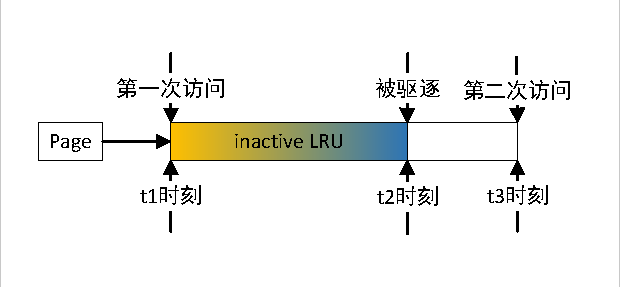
\includegraphics[width=0.5\textwidth]{重用距离.pdf}
  \caption{重用距离示意图}
  \label{fig:refault_distance}
\end{figure}


如图\ref{fig:refault_distance}所示,页面重用距离可直观理解为页面两次连续访问之间访问过的其他不同页面的数量,图中即为\(t_1\)到\(t_3\)之间被访问的不同页面数目。通过分析页面重用距离的分布,可以识别出访问模式的改变,从而及时调整页面替换策略。然而,在大规模系统中,精确计算每个页面的重用距离会引入较大的空间和计算开销,限制了其实际应用。为此,本研究提出了一种基于页面在活动链表和非活动链表间迁移行为的近似策略,通过观察页面在链表中的位置变化来间接推断其访问频度。当页面在非活动链表上被替换(即被驱逐)时,如果它在短期内再次被访问(即发生缺页异常),则说明在两次访问之间,系统至少经历了与非活动链表长度相当数量的页面访问。因此,可以通过统计缺页异常的次数和间隔来近似估计页面的访问频率。

\subsection{重用距离的近似推导}

为了简化分析,首先假设非活动链表长度固定,并且暂不考虑活动链表向非活动链表的页面降级。此简化使得非活动链表中页面的替换和访问行为更易于形式化分析。图\ref{fig:现象1}与图\ref{fig:现象2}展示了两种核心场景。

\begin{figure}[htbp]
  \centering
  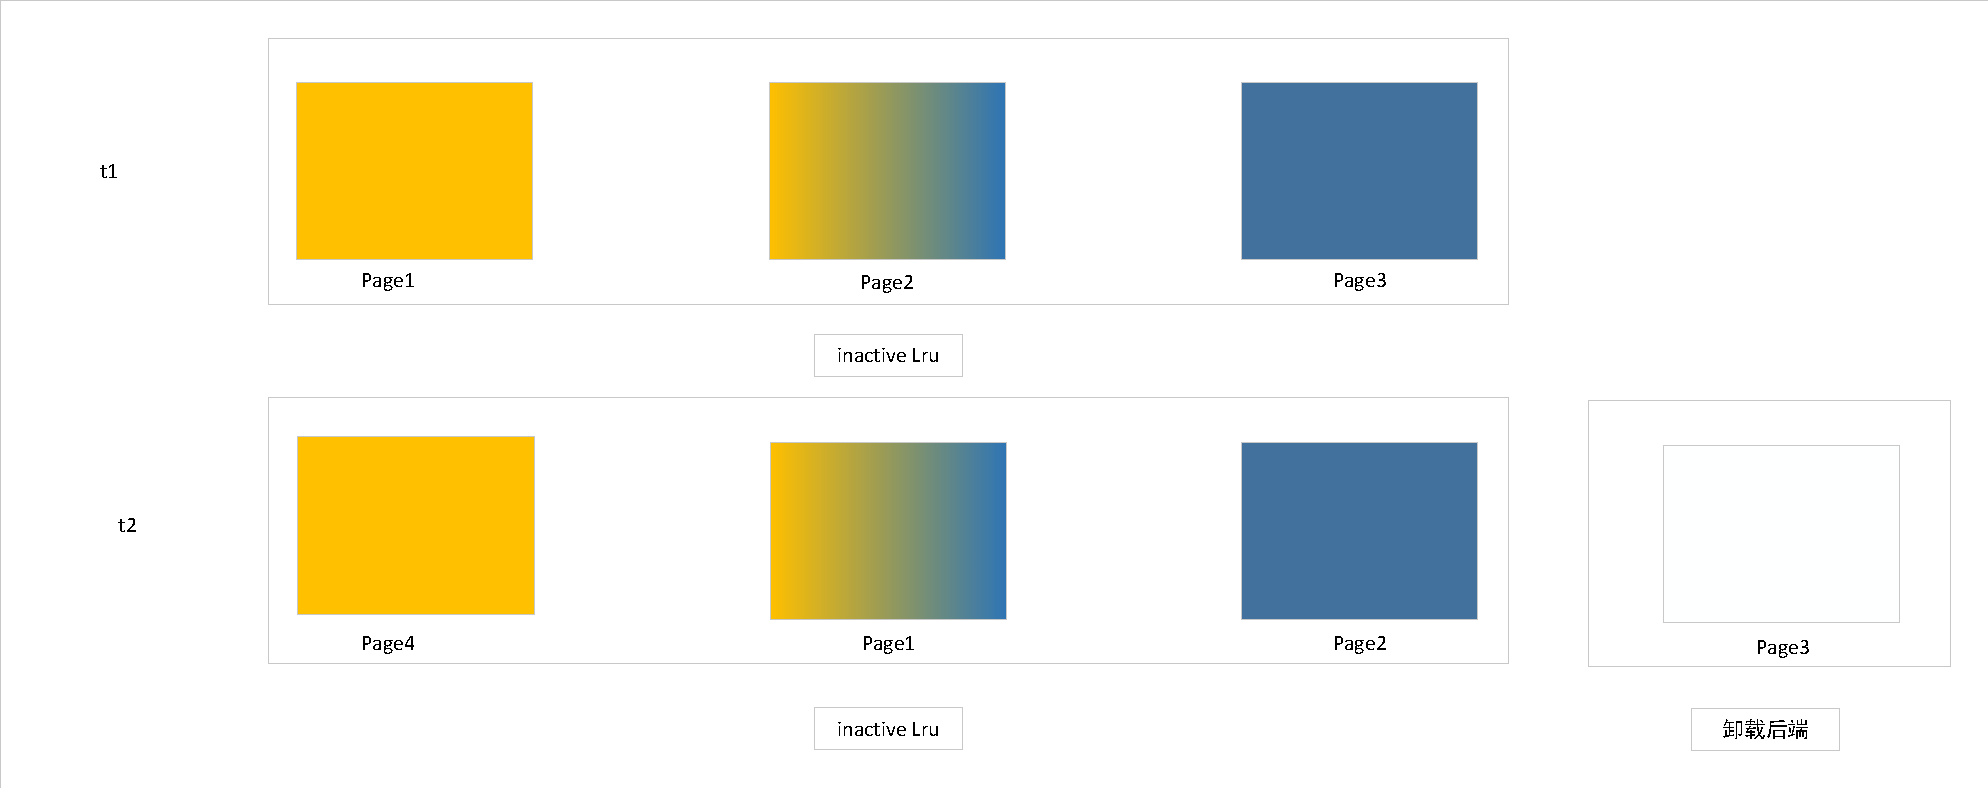
\includegraphics[width=0.5\textwidth]{现象1.pdf}
  \caption{场景一:页面首次插入非活动链表}
  \label{fig:现象1}
\end{figure}

\begin{figure}[htbp]
  \centering
  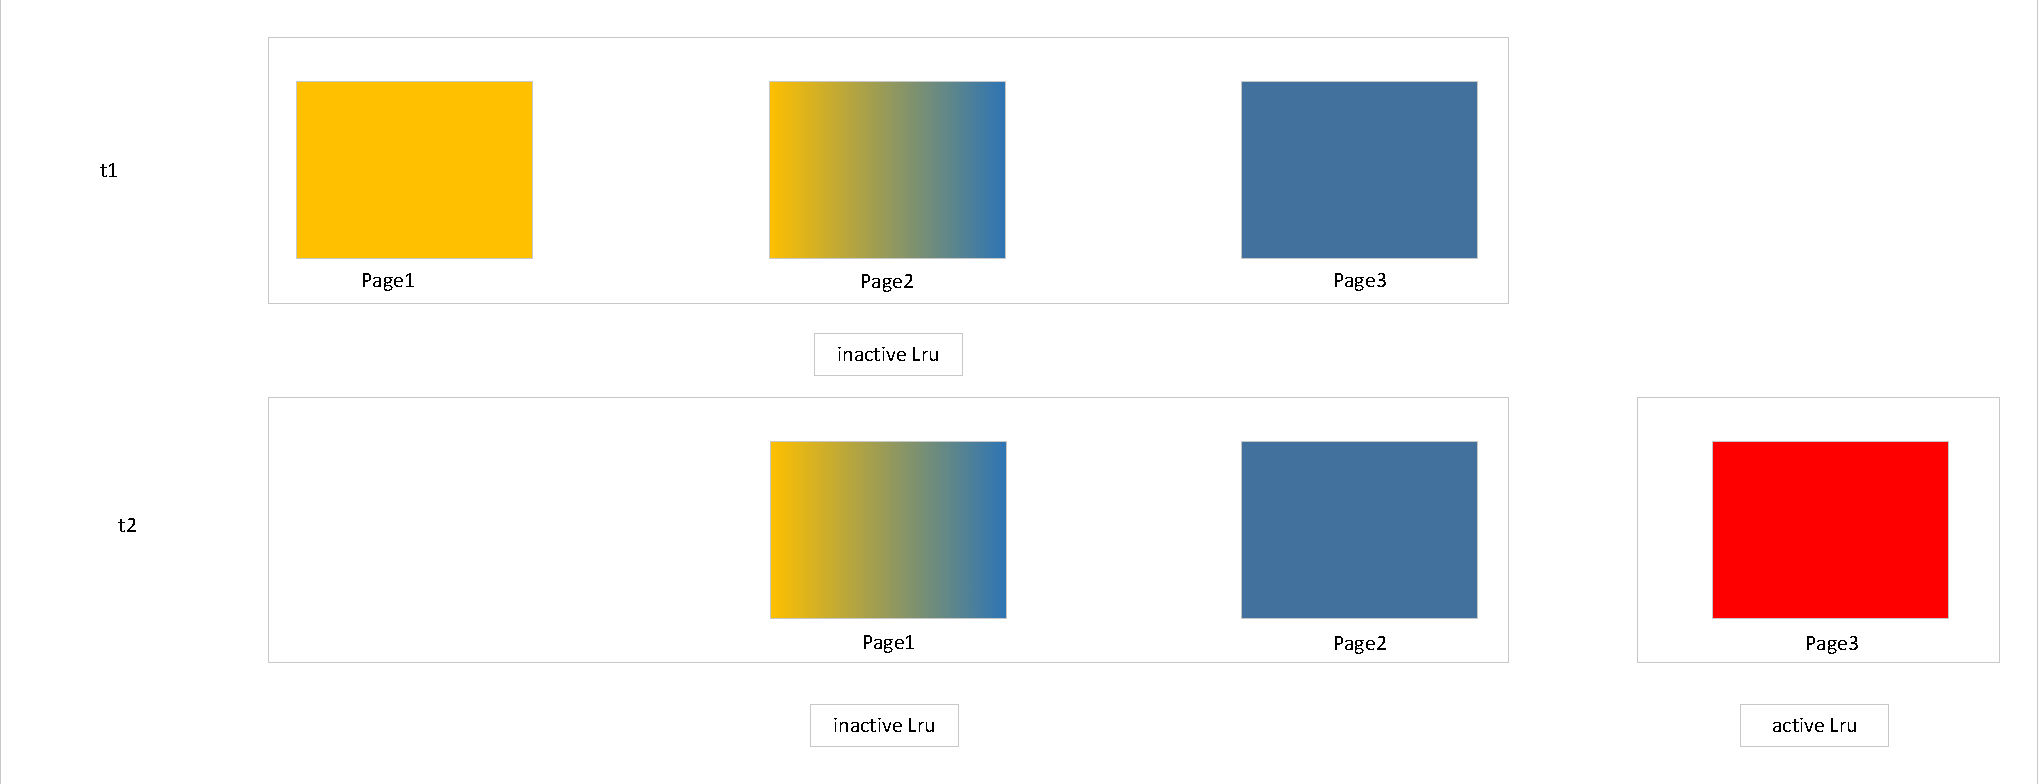
\includegraphics[width=0.5\textwidth]{现象2.pdf}
  \caption{场景二:页面在非活动链表上再次被访问并提升到活动链表}
  \label{fig:现象2}
\end{figure}

\textbf{场景一}(图\ref{fig:现象1})描述了页面首次被访问并插入到非活动链表头部。由于链表长度固定,原链表中的页面整体向尾部移动,最末尾的页面被驱逐出内存。

\textbf{场景二}(图\ref{fig:现象2})描述了页面在非活动链表上再次被访问后,被提升到活动链表。与此同时,所有比被提升页面更晚进入非活动链表的页面均向尾部移动,更接近被驱逐的状态。

在时间区间\([t_1, t_2]\)内,非活动链表上的页面只可能有两种状态:被驱逐(表明至少加载了一个新的页面)或被提升至活动链表(表明被再次访问)。令\(E(t_1,t_2)\)表示该区间内的驱逐次数,\(A(t_1,t_2)\)表示该区间的页面提升次数。由于每次驱逐对应至少一次新页面的载入,每次提升对应至少一次对非活动链表中页面的访问,因此可以合理地认为,在\([t_1,t_2]\)时间段内发生的页面访问总数\(V(t_1, t_2)\)满足以下不等式:
\[
V(t_1, t_2) \ge E(t_1,t_2) + A(t_1,t_2)
\]

这个不等式给出了页面访问次数的下界估计。

在真实系统中,还需要考虑一直停留在活动链表、从未降级的页面访问量。然而,对于访问极频繁的页面,由于它们并不会进入非活动链表,无需担心其再次访问情形的遗漏,因此对这部分页面的统计影响相对有限。

当页面\(p\)被驱逐时,记录其驱逐时刻\(t_1\)对应的全局计数器\(\mathrm{count}(t_1)\),该计数器累积了系统自启动以来的总驱逐次数和提升次数。

若该页面于时刻\(t_2\)再次被访问,则同样记录\(\mathrm{count}(t_2)\)。此时,基于上述计数器,定义页面\(p\)的重用距离为:
\begin{align}
  \label{eq:refault_distance}
  RD_{\mathrm{refault}}(p)
  &= 
  \mathrm{count}(t_2)
  \;-\;
  \mathrm{count}(t_1).
\end{align}

该距离衡量了页面从被驱逐到再次访问期间,系统所经历的页面访问次数的下界。

由于页面在非活动链表中从头部移动到尾部直至被驱逐的过程,可以近似看作是经历了一系列其他页面的访问,因此,非活动链表的长度\(L_{\mathrm{inactive}}\)可以作为页面在缓存中停留期间所经历的页面访问次数的估计。综合考虑页面在非活动链表中的移动和缺页异常期间的访问,可以得到页面\(p\)的总访问距离的近似形式:
\begin{align}
  \label{eq:dtotal}
  RD_{\mathrm{total}}(p)
  &= 
  L_{\mathrm{inactive}}
  \;+\;
  \bigl(\mathrm{count}(t_2) \;-\; \mathrm{count}(t_1)\bigr).
\end{align}

当非活动链表长度较小时,\(\mathrm{count}(t_2) - \mathrm{count}(t_1)\)的增量会相对较大。这一现象可以从页面回收机制的角度理解:非活动链表长度较小意味着页面从进入非活动链表到被驱逐的时间间隔更短,系统内存压力更大,页面更容易被换出。在这种情况下,即使是访问频率相对较高的页面也可能在短时间内被驱逐,导致它们在被驱逐后很快又被访问,从而产生更多的缺页异常和更大的\(\mathrm{count}(t_2) - \mathrm{count}(t_1)\)值。因此,这种情况下页面需要具有更高的访问频率才能在非活动链表中停留足够长的时间而不被快速驱逐。

\subsection{替换决策与回收策略}

为了确定页面是否应该继续保留在内存中,需要综合考虑其在非活动链表中的重用距离和活动链表的长度。如果页面希望继续留在内存中,其总访问距离不应超过活动链表和非活动链表的总长度:
\begin{align}
  \label{eq:active_condition_1}
  L_{\mathrm{inactive}}
  \;+\;
  \bigl(\mathrm{count}(t_2) \;-\; \mathrm{count}(t_1)\bigr)
  &\;\;\le\;\;
  L_{\mathrm{inactive}}
  \;+\;
  L_{\mathrm{active}}
\end{align}

化简后可得:
\begin{align}
  \label{eq:active_condition}
  \mathrm{count}(t_2) - \mathrm{count}(t_1)
  \;\le\;
  L_{\mathrm{active}}
\end{align}

这意味着,只有当页面的重用距离小于等于活动链表长度时,才认为其访问频率足够高,值得继续保留在内存中。

在Linux内核中,可以将该方法与\(\mathrm{swappiness}\)等内核参数结合,动态调整文件页与匿名页的回收策略。例如:
\begin{equation}
  \label{eq:swappiness1}
  \mathrm{swappiness} = \min \left( \mathrm{swappiness} \times (1 + \mathrm{refault\_active}), \; 150 \right)
\end{equation}

其中,\(\mathrm{refault\_active}\)表示在最近一段时间内页面发生缺页异常的比例,通过该值可以对回收过程进行动态调节。当系统检测到较高的文件页面refault发生时,表明当前文件页的回收策略过于激进,可能错误地驱逐了热页面,此时应适当增加\(\mathrm{swappiness}\)值以提高文件页的保留优先级。

综上所述,本研究提出的基于重用距离近似估计的页面替换策略,能够在较低开销下有效识别冷热页面,并指导文件页和匿名页的回收决策,从而提高内存利用率和系统整体性能。

\subsection{基于阴影条目的重用距离追踪内核实现}

前文提出的基于重用距离的冷热页面识别与自适应回收算法,需要在内核中实现多个关键机制以支持其运行。本节将详细介绍全局计数维护、页面驱逐与再加载的处理流程,以及阴影条目的重用机制。

\subsubsection{全局计数维护}

为了实现基于重用距离的页面替换策略,需要在内核中维护以下关键计数信息:

\begin{enumerate}
  \item 全局的驱逐和提升次数之和(记为\(nr\_count\))。
  \item 上次缺页异常统计的次数之和(记为\(nr\_refault\_last\))。
  \item 当前时刻累积的缺页异常次数之和(记为\(nr\_refault\))。
  \item 文件页面被驱逐时对应的驱逐与提升次数之和。
\end{enumerate}

其中,前三项计数直接存储在 lruvec 结构体的原子变量中,随着 lruvec 的初始化过程被设置为0。每当页面发生驱逐或提升事件时,为了保证并发访问时的计数准确性,需要对 nr\_count 执行原子递增操作。当页面再次加载时,如果满足公式\ref{eq:active_condition}的条件,则表明该页面在被驱逐后不久即被再次访问,此时系统会将其视为一次缺页异常,并相应地增加 nr\_refault 计数。通过计算 nr\_refault 和 nr\_refault\_last 的差值,可以动态评估文件页的 refault\_active ,进而通过公式\ref{eq:swappiness1}调整文件页和匿名页的回收比例。

\subsubsection{基于阴影条目的重用距离追踪机制}

为了实现基于重用距离的页面替换策略,核心挑战在于:如何在页面被驱逐后,仍能记录其驱逐时刻的全局计数值\(\mathrm{count}(t_1)\),以便在页面再次载入时计算重用距离?直接为每个被驱逐的页面单独分配存储空间记录这些信息显然不现实,这将带来大量额外的内存开销和复杂的生命周期管理问题。

本研究的关键创新在于发现了一种零额外内存开销的解决方案:复用Linux内核page cache中前缀树(Radix Tree)的数据结构特性。这一方案基于以下两个关键观察:

\begin{enumerate}
  \item 在Linux内核中,当页面被驱逐后,其在前缀树中的槽位(slot)将变为空闲状态。
  \item  struct page 指针在内存中是按照16字节对齐的,这意味着指针的低4位始终为0,其中低2位可以安全地用作标志位而不影响指针的寻址功能。
\end{enumerate}

基于上述观察,我们设计了阴影条目(shadow entry)机制:当页面被驱逐时,不是简单地将其前缀树槽位清空,而是将当前的全局计数值(\(\mathrm{count}(t_1)\))左移两位后存入该槽位,并将低两位设置为 10 标志,表示这是一个阴影条目而非有效页面指针。这样,阴影条目既保存了页面驱逐时的关键信息,又不需要额外的内存分配。

\begin{figure}[htbp]
  \centering
  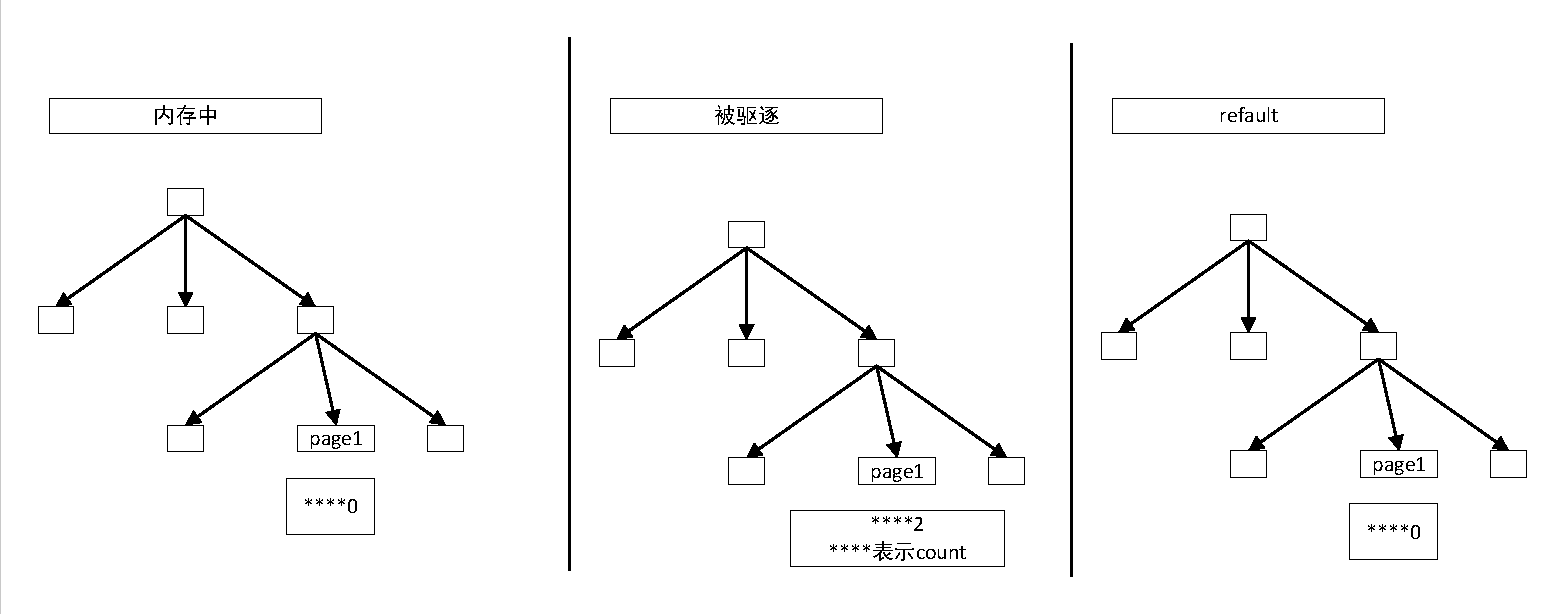
\includegraphics[width=\textwidth]{复用.pdf}
  \caption{阴影条目机制:利用前缀树指针槽位复用存储驱逐时的全局计数值}
  \label{fig:复用}
\end{figure}

如图\ref{fig:复用}所示,阴影条目机制在页面生命周期的不同阶段有三种状态:
\begin{itemize}
  \item 当页面在内存中时,前缀树槽位存储指向 struct page 的正常指针(标志位 00 )
  \item 页面被驱逐后,槽位转变为阴影条目,存储驱逐时的全局计数值(标志位 10 )
  \item 当页面再次加载的时候,阴影条目被读取并用于计算重用距离
\end{itemize}


在具体实现层面,阴影条目机制涉及以下关键步骤:

在页面驱逐阶段(\_\_remove\_mapping函数中):
\begin{enumerate}
  \item 原子读取当前全局计数器\(\mathrm{nr\_count}\)的值
  \item 将计数器值左移两位,为标志位预留空间
  \item 通过按位或操作设置低两位为 10 ,生成阴影条目
  \item 将阴影条目存入前缀树对应槽位,替换原页面指针
  \item 原子递增全局计数器\(\mathrm{nr\_count}\),记录驱逐事件
\end{enumerate}

在页面再次加载阶段(pagecache\_get\_page函数中):
\begin{enumerate}
  \item 检查前缀树槽位的低两位,判断是否为阴影条目( 10 )
  \item 若为阴影条目,提取存储的计数值(右移两位)作为\(\mathrm{count}(t_1)\)
  \item 获取当前全局计数器值作为\(\mathrm{count}(t_2)\)
  \item 根据公式\ref{eq:active_condition}判断页面是否应提升至活动链表
  \item 更新相关统计计数并清除阴影条目,替换为新加载页面的指针
\end{enumerate}

这种设计巧妙地利用了指针对齐的特性,在不增加内存开销的情况下,实现了对页面重用距离的有效追踪。通过阴影条目存储的历史信息,系统能够识别哪些页面在驱逐后迅速被再次访问(热页面),从而优化页面替换策略,提高内存利用效率。


\subsubsection{Shrinker回收机制}

在上一节中,介绍了如何通过重用前缀树指针的低位标志位来存储页面驱逐时的全局计数器值。然而,这种方法会导致前缀树中的阴影条目数量不断累积。如果不及时清理这些阴影条目,可能会导致前缀树过度膨胀,占用过多的内存资源。
\begin{table}[htbp]
  \centering
  \caption{struct shrink\_control 结构体主要字段说明}
  \label{tab:shrink_control_struct}
  \begin{tabular}{ccc}
    \toprule
    \textbf{成员} & \textbf{类型} & \textbf{说明} \\
    \midrule
    gfp\_mask & gfp\_t & 本次内存分配的掩码,指示约束条件 \\
    nid & int & 所在的 NUMA 节点 \\
    nr\_to\_scan & unsigned long & 期望本轮扫描并回收的对象数 \\
    nr\_scanned & unsigned long & 实际扫描对象数量 \\
    memcg & struct mem\_cgroup * & 针对特定 memcg 的回收(若有) \\
    \bottomrule
  \end{tabular}
\end{table}

为了解决阴影条目累积导致的内存浪费问题,本研究利用Linux内核提供的Shrinker机制来实现对阴影条目的自动回收。Shrinker是Linux内核内存回收子系统中的统一回调接口,用于管理内核缓存对象(如inode、dentry等)的回收。
\begin{table}[htbp]
  \centering
  \caption{struct shrinker 结构体主要字段说明}
  \label{tab:shrinker_struct}
  \begin{tabular}{ccc}
    \toprule
    \textbf{成员} & \textbf{类型} & \textbf{说明} \\
    \midrule
    count\_objects & 函数指针 & 返回可回收对象数,若无可回收则返回 SHRINK\_EMPTY \\
    scan\_objects & 函数指针 & 实际扫描并回收对象,返回已释放数量 \\
    batch & long & 每次回收的批次大小,默认为 0(使用默认值) \\
    seeks & int & 反映对象重建开销,影响回收优先级 \\
    flags & unsigned & Shrinker 能力标志(NUMA 感知等) \\
    list & struct list\_head & 内核内部使用,用于将 shrinker 链接到全局列表 \\
    id & int & 在 memcg 上下文中的 shrinker 标识 \\
    nr\_deferred & atomic\_long\_t * & 延迟对象数计数 \\
    \bottomrule
  \end{tabular}
\end{table}
Shrinker机制通过struct shrink\_control(表\ref{tab:shrink_control_struct})与struct shrinker(表\ref{tab:shrinker_struct})两个核心数据结构向回收框架注册接口。内核在低内存或内存压力较大时主动调用已注册的shrinker接口,以回收可释放的内核缓存对象。


本研究实现的 scan\_objects 函数利用了Linux内核现有的LRU链表机制实现高效回收。如图\ref{fig:shrink}所示,它不直接遍历整个前缀树,而是只操作已被添加到专用LRU链表的仅包含阴影条目的前缀树节点。为了避免回收操作对正常页面访问造成影响,只有当一个前缀树节点完全由阴影条目组成时,才会被添加到专用的LRU链表中进行回收。由于LRU链表提供了按访问顺序排列的节点列表,因此可以在\(O(1)\)时间内找到最近最少使用的纯阴影节点。

\begin{figure}[htbp]
  \centering
  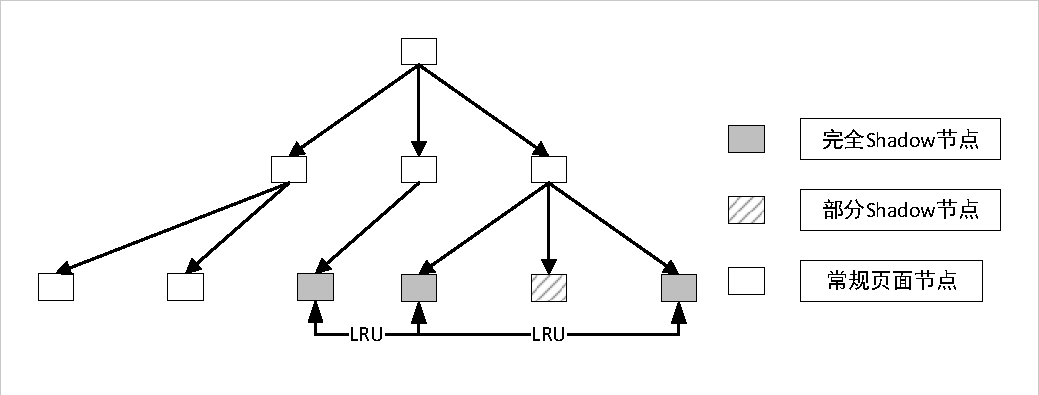
\includegraphics[width=\textwidth]{Shrinker设计.pdf}
  \caption{Shrinker机制工作原理示意图}
  \label{fig:shrink}
\end{figure}
 count\_objects 函数负责估算可回收的阴影条目数量。它根据系统当前的内存压力水平,动态计算合理的阴影节点数量上限,并只回收超出这一上限的节点。








\section{本章小结}
\label{sec:本章小结}

本章详细介绍了基于内存压力的自适应主动冷页面卸载框架的设计与实现。首先,介绍了利用proc文件系统实现的mpfs模块,提供了用户态与内核态之间的标准交互接口。mpfs模块允许用户态程序实时获取内存压力信息,并动态调整采样周期和压力阈值,为用户态的调控策略提供了基础。随后,提出了基于内存压力的动态调控模型,利用负反馈机制,根据实时内存压力动态调整内存使用范围,实现了主动的冷页面卸载。该模型通过参数化设计,可以灵活适应不同的应用场景和性能需求。最后,详细介绍了基于重用距离的自适应页面回收策略。通过近似计算页面的重用距离,实现了文件页和匿名页的自适应平衡回收。为了支持该策略,本研究在内核中实现了全局计数维护、阴影条目管理和Shrinker回收机制。通过重用前缀树指针的低位标志位,避免了在 struct page 结构中引入额外字段,最大程度地减少了内存开销。

本章提出的框架和算法,为实现高效、自适应的内存管理提供了可行的方案。通过将内存压力作为核心调控指标,结合重用距离进行页面回收决策,能够在保证系统性能的同时,显著提高内存资源的利用率。未来的研究方向包括引入机器学习技术实现参数的自适应调整,以及将该模型扩展至更广泛的资源管理领域。
